\subsection{Đề 01}
\Opensolutionfile{ans}[ans/ans-CTST-0-OTGK1-De07-LC]
\caulc
\begin{ex}%[0D1N1-5]
	Mệnh đề \lq\lq $\forall x\in \mathbb{R},\,\,x^2-x+3<0$ \rq\rq có mệnh đề phủ định là
	\choice
	{\True  \lq\lq $\exists x \in \mathbb{R},\,\,x^2-x+3\ge 0$ \rq\rq}
	{\lq\lq $\forall x \in \mathbb{R},\,\,x^2-x+3>0$ \rq\rq}
	{\lq\lq $\forall x \in \mathbb{R},\,\,x^2-x+3<0$ \rq\rq}
	{\lq\lq $\nexists x \in \mathbb{R},\,\,x^2-x+3<0$ \rq\rq}
	\loigiai{
		 \lq\lq $\exists x \in \mathbb{R},\,\,x^2-x+3\ge 0$ \rq\rq.}
\end{ex}
\begin{ex}%[0D1N2-1]
	Cho tập hợp $A=\{x\in \mathbb{R}|x^2+2x+8=0\}$. Số phần tử của tập $A$ là
	\choice
	{$1$}
	{$2$}
	{\True $0$}
	{$\varnothing$}
	\loigiai{
		Ta có $A=\{x\in\mathbb{R}|x^2+2x+8=0\}$.\\
		Vì phương trình $x^2+2x+8=0$ vô nghiệm nên $A=\varnothing$.}
\end{ex}
\begin{ex}%[0D1N3-1]
	Cho hai tập hợp $A=\{5;7;9;10\}$ và $B=\{2;3;5;8;9\}$. Tìm tập hợp $A\cap B$.
	\choice
	{$A\cap B=\{5;7;9\}$}
	{$A\cap B=\{2;3;8\}$}
	{$A\cap B=\{5;7\}$}
	{\True $A\cap B=\{5;9\}$}
	\loigiai{
		Ta có $A\cap B=\{5;9\}$.}
\end{ex}
\begin{ex}%[0D2N1-1]
	Bất phương trình nào sau đây là bất phương trình bậc nhất hai ẩn?
	\choice
	{$2x^2+3y>0$}
	{$x^2+y^2<2$}
	{$x+y^2\ge 0$}
	{\True $2x+3y\ge 0$}
	\loigiai{
		Bất phương trình bậc nhất hai ẩn $x$, $y$ là bất phương trình có một trong các dạng $ax+by>c$; $ax+by\ge c$; $ax+by<c$; $ax+by\le c$ $(a^2+b^2>0)$.}
\end{ex}
\begin{ex}%[0D2N2-1]
	Trong các hệ bất phương trình sau, hệ bất phương trình nào là hệ bất phương trình bậc nhất hai ẩn?
	\choice
	{ $\heva{& 4x+5y<-10 \\
			& {9^3}x+5y^2\ge 6}$ }
	{ $\heva{& x+y\le 1 \\
			& x+3y+z>2 \\
			& x-z>0} $}
	{ $\heva{& x>3 \\
			& y\le 1 \\
			& x-3y^2\ge 0}$}
	{\True $\heva{& 2x-3y<0 \\
			& 5x+3y+1\le 0}$}
	\loigiai{
		Hệ bất phương trình bậc nhất $2$ ẩn là $1$ hệ gồm $2$ hay nhiều bất phương trình bậc nhất $2$ ẩn.}
\end{ex}
\begin{ex}%[0D3N1-4]
	Cho hàm số $y=\dfrac{x+1}{x-1}$. Tìm tọa độ điểm thuộc đồ thị của hàm số và có tung độ bằng $-2$.
	\choice
	{$(0;-2)$}
	{\True $\left(\dfrac{1}{3};-2\right)$}
	{$(-2;-2)$}
	{$(-1;-2)$}
	\loigiai{
		Gọi $M_0(x_0;-2)$ là điểm thuộc đồ thị hàm số có tung độ bằng $-2$.\\
		Khi đó: $\dfrac{x_0+1}{x_0-1}=-2 \Leftrightarrow x_0+1=2\left(1-x_0\right) \Leftrightarrow 3 x_0=1 \Leftrightarrow x_0=\dfrac{1}{3} \Rightarrow M\left(\dfrac{1}{3};-2\right)$.}
\end{ex}
\begin{ex}%[0D3N1-1]
	Đồ thị của hàm số $y=f(x)=\heva{&2x+1 &\text{khi} && x\le 2\\&-3 &\text{khi} && x>2}$ đi qua điểm nào sau đây?
	\choice
	{$(0;-3)$}
	{$(3;7)$}
	{$(2;-3)$}
	{\True $(0;1)$}
	\loigiai{
		Thử lần lượt từng phương án A, B, C, D với chú ý về điều kiện ta được:\\
		$f(0)=2\cdot0+1=1 \ne-3$, đồ thị không đi qua điểm $(0;-3)$.\\
		$f(3)=-3\ne 7$, đồ thị không đi qua điểm $(3;7)$.\\
		$f(2)=2\cdot2+1=5\ne-3$, đồ thị không đi qua điểm $(2;-3)$.\\
		$f(0)=2\cdot 0+1=1$, đồ thị đi qua điểm $(0;1)$.}
\end{ex}
\begin{ex}%[0H4N1-1]
	Cho góc $\alpha \in (90^\circ;180^\circ)$, mệnh đề đúng về dấu của $\sin \alpha$ và $\cos \alpha$ là
	\choice
	{$\sin \alpha>0$, $\cos \alpha>0$}
	{\True $\sin \alpha>0$, $\cos \alpha<0$}
	{$\sin \alpha<0$, $\cos \alpha >0$}
	{$\sin \alpha<0$, $\cos \alpha <0$}
	\loigiai{
		Cho góc $\alpha \in (90^\circ;180^\circ)$, ta có $\sin \alpha >0$, $\cos \alpha<0$.}
\end{ex}
\begin{ex}%[0H4N2-1]
	Cho tam giác $ABC$ có $AB=c$, $BC=a$, $AC=b$. Hãy chọn mệnh đề \textbf{sai} trong các mệnh đề sau?
	\choice
	{$\cos A=\dfrac{b^2+c^2-a^2}{2bc}$}
	{$b\cdot\sin C=c\cdot\sin B$}
	{$\dfrac{a}{\sin A}=2R$}
	{\True $b^2=a^2+c^2+2ac\cdot\cos B$}
	\loigiai{
		Ta có $b^2=a^2+c^2-2ac\cdot\cos B$.}
\end{ex}
\begin{ex}%[0H4N3-1]
	
	Cho tam giác $ABC$ có $AB=c$, $BC=a$, $AC=b$. Gọi $p$ là nửa chu vi của tam giác, $r$ là bán kính đường tròn nội tiếp tam giác và $S$ là diện tích tam giác đó. Mệnh đề nào sau đây đúng?
	\choice
	{$S=p(p-a)(p-b)(p-c)$}
	{\True $S=pr$}
	{$S=\dfrac{abc}{4r}$}
	{$S=2bc\sin A$}
	\loigiai{Ta có $S=pr$.}
\end{ex}
\begin{ex}%[0D1H3-3]
	Cho tập $A=\{x\in \mathbb{R}|-4\le x<5\}$ và tập $B=\{x\in \mathbb{R}|-1<x\le 6\}$. Xác định tập hợp $A\cap B$.
	\choice
	{$[-4;6)$}
	{$(5;6]$}
	{$[-4;-1)$}
	{\True $(-1;5)$}
	\loigiai{
		$A=[-4;5)$,
		$B=(-1;6]$,
		$A\cap B=(-1;5)$.}
\end{ex}
\begin{ex}%[0H4H3-1]
	Tam giác $ABC$ có $AC=4$, $\widehat{BAC}=30^\circ$ , $\widehat{ACB}=75^\circ$. Tính diện tích tam giác $ABC$.
	\choice
	{ $S_{\triangle ABC}=8$}
	{ $S_{\triangle ABC}=4\sqrt{3}$}
	{\True $S_{\triangle ABC}=4$}
	{ $S_{\triangle ABC}=8\sqrt{3}$}
	\loigiai{
		Ta có $\widehat{ABC}=180^\circ -\left( \widehat{BAC}+\widehat{ACB}\right)=75^\circ =\widehat{ACB}$.\\
		Suy ra tam giác $ABC$ cân tại $A$ nên $AB=AC=4$.\\
		Diện tích tam giác $ABC$ là ${S_{\triangle ABC}}=\dfrac{1}{2}AB \cdot AC\cdot \sin \widehat{BAC}=4$.
	}
\end{ex}
\Closesolutionfile{ans}
\indapan{6}{ans/ans-CTST-0-OTGK1-De07-LC}
%-------------------------------------------
\Opensolutionfile{ans}[ans/ans-CTST-0-OTGK1-De07-DS]
\cauds
\begin{ex}%[0D1N3-1]	
	Cho hai tập hợp $A=\{a;c;d;e;f\}$ và $B=\{b;c;d;e;g;h\}$. Vậy
	\choiceTF
	{\True tập hơp $A$ có $5$ phần tử}
	{$A\subset B$}
	{\True $A\cap B=\{c;d;e\}$}
	{$A \setminus B=\{a;e\}$}	
	\loigiai{
	\begin{itemchoice}
		\itemch Đúng. Vì $A=\{a;c;d;e;f\}$ nên tập hơp $A$ có $5$ phần tử.
		\itemch Sai. Vì phần tử $a$ của tập hợp $A$ không là phần tử của tập hợp $B$.
		\itemch Đúng. Vì $A cap B=\{ c;d;e\}$.
		\itemch Sai. Vì $A\setminus B=\{a;f\}$.
	\end{itemchoice}}
\end{ex}
\begin{ex}%[0D2V2-2]
	Cho hệ bất phương trình $\heva{&3x+2y\ge 9\\&x-2y\le 3\\&x+y\le 6\\&x \ge 1}\quad(I)$. Khi đó
	\choiceTF
	{\True Miền nghiệm của hệ bất phương trình là miền tứ giác}
	{\True $(3;1)$ là một nghiệm của hệ bất phương trình}
	{$x=1$, $y=3$ là nghiệm của hệ bất phương trình $(I)$ sao cho $F=3x-y$ đạt giá trị lớn nhất}
	{\True $x=1$, $y=5$ là nghiệm của hệ bất phương trình $(I)$ sao cho $F=3x-y$ đạt giá trị nhỏ nhất}
	\loigiai{
		\begin{itemchoice}
			\itemch  Đúng. Vì miền nghiệm của hệ $(I)$ là miền tứ giác $ABCD$ với $A(3;0)$, $B(5;1)$, $C(1;5)$, $D(1;3)$.
			\begin{center}
				\begin{tikzpicture}[scale=0.7, line join=round, line cap=round, >=stealth]
					\tikzset{every node/.style={scale=1}}
					\def\xmin{-3}\def\xmax{7}\def\ymin{-3}\def\ymax{8}
					\draw[->] (\xmin-0.2,0)--(\xmax+0.2,0) node[below]{$x$};
					\draw[->] (0,\ymin-0.2)--(0,\ymax+0.2) node[right]{$y$};
					\draw (0,0) node[below left]{$O$};
					\foreach \x in {1,3,5,6}\draw (\x,0.1)--(\x,-0.1) node[below]{$\x$};
					\foreach \y in {1,3,5,6}\draw (0.1,\y)--(-0.1,\y) node[above left]{$\y$};
					\clip (\xmin,\ymin) rectangle (\xmax,\ymax);
					\draw[thick,smooth,samples=200,domain=\xmin:\xmax] plot (\x,{(-3/2)*(\x)+(9/2)});
					\clip (\xmin,\ymin) rectangle (\xmax,\ymax);
					\draw[thick,smooth,samples=200,domain=\xmin:\xmax] plot (\x,{(1/2)*(\x)-(3/2)});
					\draw[thick,smooth,samples=200,domain=\xmin:\xmax] plot (\x,{-1*(\x)+6});
					\draw[thick,smooth,samples=200,domain=\xmin:\xmax] (1,-3) -- (1,8);
					\fill[pattern=north east lines,smooth]
					plot[domain=-3:7] (\x,{(-3/2)*(\x)+(9/2)})
					-- plot[domain=7:-3] (\x,{0*(\x)-5})
					-- cycle;
					\fill[pattern=north east lines,smooth]
					plot[domain=-3:7] (\x,{(1/2)*(\x)-(3/2)})
					-- plot[domain=7:-3] (\x,{0*(\x)-5})
					-- cycle;
					\fill[pattern=north east lines,smooth]
					plot[domain=-3:7] (\x,{0*(\x)+8})
					-- plot[domain=7:-3] (\x,{-1*(\x)+6})
					-- cycle;
					\fill[pattern=north east lines,smooth]
					plot[domain=-3:1] (\x,{0*(\x)+8})
					-- plot[domain=1:-3] (\x,{0*(\x)-3})
					-- cycle;
					\path
					(1,5) node[above right]{$A$}
					(1,3) node[above right]{$B$}
					(3,0) node[above]{$C$}
					(5,1) node[above]{$D$}
					;
				\end{tikzpicture}
			\end{center}
			\itemch  Đúng. Vì $(3;1)$ là một nghiệm của hệ bất phương trình.
			\itemch Sai. Vì giá trị của $F=3x-y$ tại các cặp số $(x;y)$ là toạ độ của các đỉnh tứ giác $ABCD$ rồi so sánh các giá trị đó, ta được $F$ đạt giá trị lớn nhất bằng $14$ tại $x=5$, $y=1$.
			\itemch  Đúng. Vì $F$ đạt giá trị nhỏ nhất bằng $-2$ tại $x=1$, $y=5$.
		\end{itemchoice}
	}
\end{ex}
\begin{ex}%[0D3H1-4]
 Cho hàm số ${y=f(x)}$ có đồ thị là đường gấp khúc như hình bên dưới.
\begin{center}
	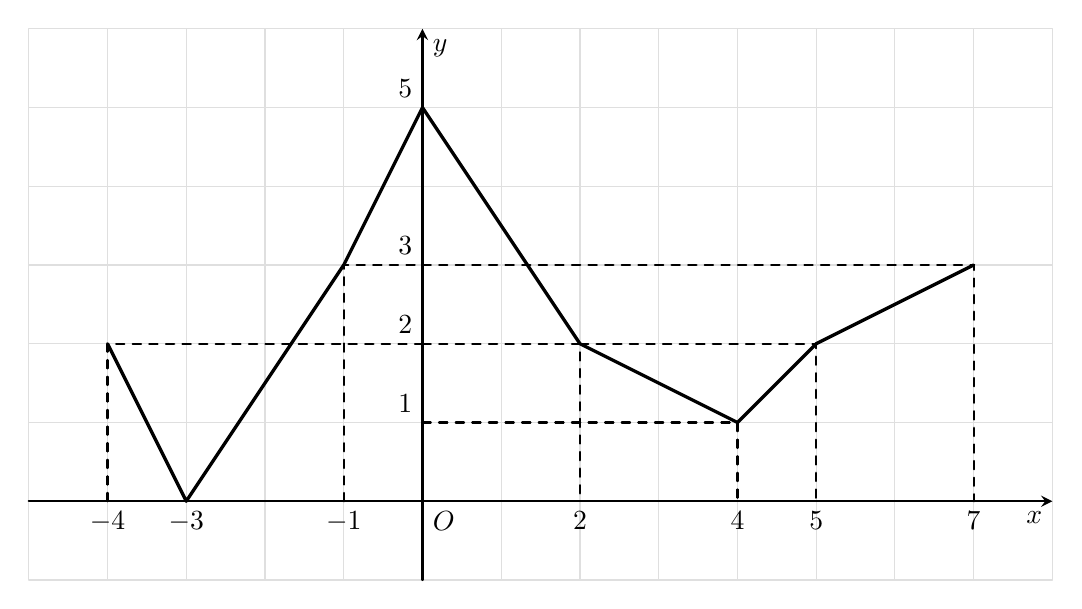
\begin{tikzpicture}[line join=round, line cap=round,thick]
	\draw[gray!50,thin,opacity=.5]
	(-5,-1) grid (8,6);
	\draw [-stealth,thick](-5,0) -- (8,0) node[below left]{$x$};
	\draw [-stealth,thick](0,-1) -- (0,6) node[below right]{$y$};
	\draw[very thick] (-4,2)--(-3,0)--(-1,3)--(0,5)--(2,2)--(4,1)--(5,2)--(7,3)	; 
	\draw[dashed] (-4,0) node[below]{$-4$}|-(0,2) node[above left]{$2$}
	(-1,0) node[below]{$-1$}|-(0,3) node[above left]{$3$}
	(0,2)-|(2,0) node[below]{$2$}
	(0,1) node[above left]{$1$}-|(4,0) node[below]{$4$}
	(2,2)--(5,2)--(5,0) node[below]{$5$}
	(0,3)-|(7,0) node[below]{$7$}
	(0,0) node[below right]{$O$}
	(-3,0) node[below]{$-3$}
	(0,5) node[above left]{$5$}
	;
\end{tikzpicture}
\end{center}
Khi đó
	\choiceTF
	{Tập giá trị hàm số $T=[-4;7]$}
	{\True Ta thấy điểm $(-4;2)$, $(4;1)$ thuộc đồ thị hàm số, điểm $(2;3)$ không thuộc đồ thị hàm số}
	{\True Ta có $f(-1)=3$, $f(5)=2$}
	{\True Hàm số đã cho đồng biến trên các khoảng $(-3;0)$, $(4;7)$; hàm số nghịch biến trên các khoảng $(-4;-3)$, $(0;4)$}
	\loigiai{
		\begin{itemchoice}
			\itemch Sai. Tập xác định hàm số $\mathscr{D}=[-4;7]$. Tập giá trị hàm số $T=[0;5]$. 
			\itemch Đúng. Ta thấy điểm $(-4;2)$, $(4;1)$ thuộc đồ thị hàm số, điểm $(2;3)$ không thuộc đồ thị hàm số.
			\itemch Đúng. Ta có: $f(-1)=3$, $f(5)=2$.
			\itemch Đúng. Hàm số đã cho đồng biến trên các khoảng $(-3;0)$, $(4;7)$; hàm số nghịch biến trên các khoảng $(-4;-3)$, $(0;4)$.
		\end{itemchoice}
	}
\end{ex}
\begin{ex}%[0H4H2-1]
	Cho tam giác ${ABC}$ biết $a=3$ cm, $b=4$ cm, $\widehat{C}=30^{\circ}$. Khi đó
	\choiceTF
	{\True $c^2=a^2+b^2-2ab \cos C$}
	{ $c\approx 3{,}05$ cm}
	{\True $\cos A\approx 0{,}68$}
	{$\widehat{B}\approx 77{,}2^\circ$}
	\loigiai{
		\begin{itemchoice}
		\itemch Đúng. Áp dụng định lí côsin trong tam giác, ta có: $c^2=a^2+b^2-2ab \cos C$. 
		\itemch Sai. Ta có: $c^2=3^2+4^2-2\cdot 3\cdot 4\cos 30^{\circ}=25-12 \sqrt{3}$. Do đó, $c \approx 2{,}05$ (cm). 
		\itemch Đúng. Ta có: $a^2=b^2+c^2-2bc\cos A$\\
		 $\Rightarrow \cos A=\dfrac{b^2+c^2-a^2}{2bc}=\dfrac{4^2+(25-12 \sqrt{3})^2-3^2}{2\cdot 4\sqrt{25-12\sqrt{3}}}
		 \approx 0,68$.
		\itemch Sai. Vì $\widehat{A} \approx 47{,}2^{\circ}$. Do đó, $\widehat{B}=180^{\circ}-\widehat{A}-\widehat{C}=180^{\circ}-47{,}2^{\circ}-30^{\circ}=102{,}8^{\circ}$.
	\end{itemchoice}
	}	
\end{ex}
\Closesolutionfile{ans}
\indapan{3}{ans/ans-CTST-0-OTGK1-De07-DS}
%-------------------------------------------
\Opensolutionfile{ans}[ans/ans-CTST-0-OTGK1-De07-KQ]
\caukq
\begin{ex}%[0D2H1-3]
	Bạn Minh để dành được $900$ nghìn đồng. Trong một đợt ủng hộ trẻ em mồ côi, Minh đã lấy ra $x$ tờ tiền loại $50$ nghìn đồng, $y$ tờ tiền loại $100$ nghìn đồng để trao tặng. Một bất phương trình mô tả điều kiện ràng buộc đối với $x$, $y$ là $ax+by\le c$. Khi đó $c-a-b$ bằng
	\shortans{$750$}
	\loigiai{
		Tổng số tiền bạn Minh đã lấy để trao tặng: $50x+100y$ (nghìn đồng).\\
		Mà Minh để dành được $900$ nghìn đồng nên $50x+100y\le 900$.\\
		Vậy $a=50$, $b=100$, $c=900$ nên $c-a-b=750$
	}
\end{ex}
\begin{ex}%[0D2V2-3]
		Một gia đình dự định trồng rau và hoa trên một mảnh đất có diện tích $8$ ha. Nếu trồng $1$ ha rau thì cần $20$ ngày công và thu lợi $3$ triệu. Nếu trồng hoa thì cần $30$ ngày công và thu lợi $4$ triệu. Biết rằng, gia đình chỉ có thể sử dụng không quá $180$ ngày công cho công việc trồng rau và hoa. Tìm số lợi nhuận cao nhất từ việc gia đình trồng rau và hoa nói trên.
	\shortans{$26$}
	\loigiai{
	Gọi $x$, $y$ $(x\ge 0$, $y\ge 0)$ lần lượt là số ha đất trồng rau và hoa.\\
	Diện tích đất trồng canh tác không vượt quá $8$ ha nên ta có: $x+y\le 8$.\\
	Số ngày công sử dụng không vượt quá $180$ ngày nên $20x+30y\le 180$.\\
	Từ đó, ta có hệ bất phương trình
	 $\heva{& x\ge 0  \\ 
	 	    & y\ge 0 \\ 
	 	    & x+y\le 8 \\ 
	 	    & 20x+30y\le 180}\quad(1) $ \\
	Ta cần tìm $x$, $y$ sao cho $T(x,y)=3x+4y$ lớn nhất. \\
	Miền nghiệm của hệ $(1)$ được biểu diễn như sau
\begin{center}
	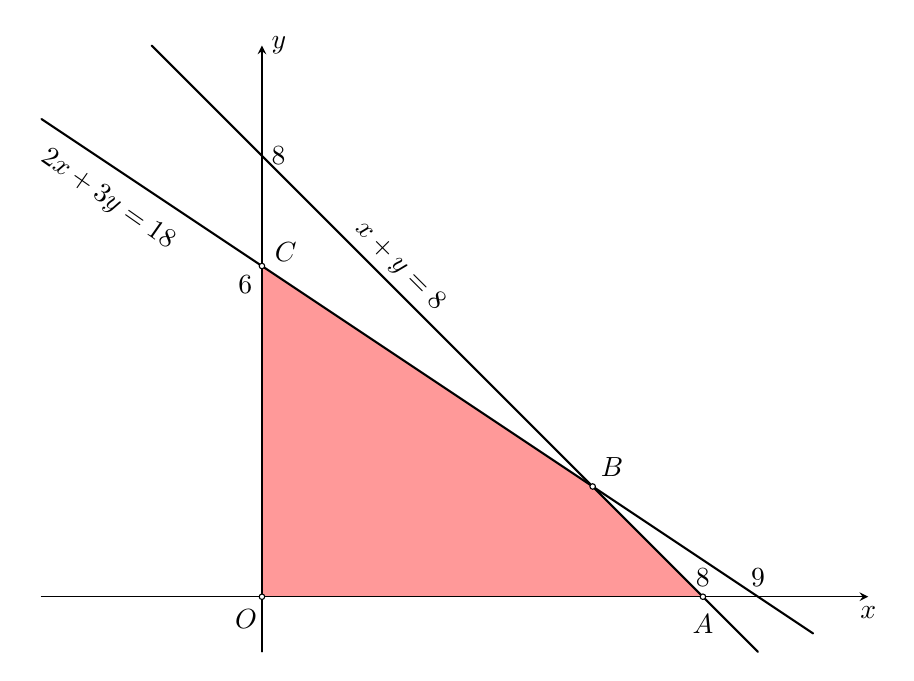
\begin{tikzpicture}[scale=0.7, line join=round, line cap=round,>=stealth]
		\path 	(0,0) coordinate (O)
		(8,0) coordinate (A)
		(6,2) coordinate (B)
		(0,6) coordinate (C)
		(9,0) coordinate (D)
		(0,8) coordinate (E);
		\fill[red!40] (O) -- (A) -- (B) -- (C) -- cycle;
		\draw[->] (-4,0) -- (11,0) node[below]{$x$};
		\draw[->](0,-1)--(0,10) node[right]{$y$};
		\draw[smooth,samples=100,black,line width=0.75] plot[domain=-2:9](\x,{-1*(\x)+8});
		\draw[smooth,samples=100,black,line width=0.75] plot[domain=-4:10](\x,{-2/3*(\x)+6});
		\foreach \x/\g in {A/-90,B/45,C/30,O/235}
		\draw [fill=white]  (\x) circle (0.05) + (\g:0.5) node {$\x$};	
		\draw (A) node[above] {$8$}
		(D) node[above] {$9$}
		(E) node[right] {$8$}
		(C) node[below left] {$6$}
		;
		\draw (2.5,6) node {\rotatebox{-45} {$x+y=8$}}
		(-2.8,7.2) node {\rotatebox{-35} {$2x+3y=18$}}
		;
	\end{tikzpicture}
\end{center}
	Miền nghiệm của hệ bất phương trình trên là miền trong của tứ giác $OABC$, kể cả $4$ cạnh của tứ giác đó, với $O(0;0)$, $A(8;0)$, $B(6;2)$, $C(0;6)$.\\
	Ta có: $T(0;0)=0$; $T(8;0)=21$; $T(6;2)=26$; $T(0;6)=24$.\\
	Vậy số lợi nhuận cao nhất mà gia đình thu được từ trồng rau và hoa là $26$ triệu đồng.
	}
\end{ex}
\begin{ex}%[0D3H1-7]
		Một hãng taxi có bảng giá như sau (sử dụng cho taxi $4$ chỗ)
	\begin{center}
		\begin{tabular}{|c|c|c|}
			\hline
			\textbf{Giá mở cửa (0{,}5km)} & \textbf{Giá cước các km tiếp theo} & \textbf{Giá cước từ km thứ 31} \\
			\hline
			11 000 đồng & 14 500 đồng/km & 11 600 đồng/km \\
			\hline
		\end{tabular}
	\end{center}
	Bạn Trân bắt taxi đi quãng đường $35$ km thì phải trả số tiền là bao nhiêu nghìn đồng (kết quả làm tròn đến hàng nghìn).
	\shortans{$497$}
	\loigiai{
		Gọi $x$ là số km cần đi $(x\ge 0)$. Gọi $f(x)$ là số tiền phải trả khi đi $x$ km. Ta có:\\
		Nếu $0<x\le 0{,}5$ thì $f(x)=11\,000$\\
		Nếu $0{,}5<x\le 30$ thì $f(x)=1\,1000+14\,500(x-0{,}5)=3\,750+14\,500x$.\\
		Nếu $x>30$ thì $f(x)=11\,000+14\,500(30-0{,}5)+11\,600(x-30)=90\,750+11\,600x$.\\
		Vậy ta có công thức hàm $f(x)$ như sau
			\[f(x)=\heva{&11\,000 &\text{nếu} &&0<x\le 0{,}5 \\&
				3\,750+1\,400x &\text{nếu} &&0{,}5<x\le 30\\&
				90\,750+11\,600x & \text{nếu} &&x>30} 
			\]
		Vì bạn Trân muốn đi $35$ km nên $x=35>30$ nên\\ $f(35 )=90\,750+11\,600\cdot 35=496\,750$ (đồng)\\
		Vậy để đi $35$ km bạn trân phải trả $497$ nghìn đồng.
		}
\end{ex}
	\begin{ex}%[0H4H1-2]
		Cho góc $\alpha$ với $\cot \alpha=5$. Tính giá trị của biểu thức $P=2\cos^2 \alpha+5\sin \alpha \cos \alpha+1$ (kết quả làm tròn đến hàng phần trăm).
		\shortans{$3{,}89$}
		\loigiai{
		Ta có: $P={\sin^2}\alpha \left( 2{\cot^2}\alpha +5\cot \alpha +\dfrac{1}{{\sin ^2}\alpha } \right)=\dfrac{1}{1+{{\cot }^2}\alpha }\left( 3{{\cot }^2}\alpha +5\cot \alpha +1 \right)=\dfrac{101}{26}\\
		\approx 3{,}89$.
		}
	\end{ex}
	\begin{ex}%[0H4N2-1]
		Tam giác $ABC$ có $BC=10$ và $\widehat{A}=30^{\circ}$. Tính bán kính $R$ của đường tròn ngoại tiếp tam giác $ABC$.
		\shortans{10}
		\loigiai{
		Áp dụng định lí sin, ta có $\dfrac{BC}{\sin \widehat{BAC}}=2R\Rightarrow R=\dfrac{BC}{2\sin \widehat{A}}=\dfrac{10}{2\sin 30^{\circ}}=10$.
		}
	\end{ex}
	
    \begin{ex}%[0H4V3-2]
	Một người quan sát đỉnh của một ngọn núi nhân tạo từ hai vị trí khác nhau của tòa nhà. Lần đầu tiên người đó quan sát đỉnh núi từ tầng trệt với phương nhìn tạo với phương nằm ngang $35^\circ$ và lần thứ hai người này quan sát tại sân thượng của cùng tòa nhà đó với phương nằm ngang $15^\circ$ (như hình vẽ). Tính chiều cao ngọn núi biết rằng tòa nhà cao $60\,\text{m}$ (kết quả làm tròn đến hàng phần mười).
	\begin{center}
		\begin{tikzpicture}[scale=.5, font=\footnotesize, line join=round, >=stealth]
			\foreach \x/\y/\z in {0/0/O,2.2/0/A,2.2/7/B,11.27/13.13/C,11.27/7/E,11.27/0/D}
			\path (\x,\y) coordinate (\z);
			\def\nhathap{6} %so tang nha thap
			\def\dai{1} %chieu dai 1 khoi
			\def\cao{1} %chieu cao 1 khoi
			%Xay nha thap
			\newcommand{\xaynha}[2]{
				\draw[very thick,black] (#1,#2)rectangle(#1+\dai,#2+\cao);
				\draw[very thick,fill=red] (#1,#2)rectangle(#1+\dai,#2+0.25*\cao);
				\filldraw[very thick,cyan] (#1+0.2*\dai,#2+0.25*\cao)rectangle(#1+0.8*\dai,#2+0.9*\cao);
			}
			\foreach \j in {0,...,\nhathap}{
				\foreach \i in {0,1}{
					\xaynha{\i*1.1}{\j*\cao}
				}
			}
			\fill [green!60!blue] plot [smooth ] coordinates{(6.64,0)(7.36,3.91) (7.96,5.47) (8.28,4.92) (8.63,4.77)(8.84,3.99) (9.47,5.08) (9.87,7.42)(10.4,8.36)(10.37,9.77)(11.27,13.13)(11.93,12.11)(11.83,10.55)(12.44,9.14)(12.91,6.33)(12.75,4.77)(13.94,0.7)(13.78,0)};
			\draw [thick] (A)--(D)--(C);
			\draw[dashed](B)--(C)--(A) (B)--(E);
			\path pic[draw=black,angle radius = 12] {angle = D--A--C} node [shift={(1.7,.3)}]{$35^\circ$} ;
			\path pic[draw=black,angle radius = 12,double] {angle = E--B--C} node [shift={(2.2,3.8)}]{$15^\circ$} ;
			\foreach \d/\g in {A/-90, B/90, C/90,E/0,D/-90}
			\path[draw,fill=white] (\d) circle(1pt) + (\g:9pt) node {$\d$};
		\end{tikzpicture}
	\end{center}
			\shortans{$97,2$}
			\loigiai{
			Ta có: $\widehat{CBA}=\widehat{CBE}+\widehat{EBA}=90^\circ+15^\circ=105^\circ$.\\
			$\widehat{BAC}=\widehat{BAD}-\widehat{CAD}=90^\circ-35^\circ=55^\circ\Rightarrow \widehat{BCA}=180^\circ-\left( \widehat{CBA}+\widehat{BAC}\right)=20^\circ$.\\
			Áp dụng định lý sin cho $\triangle CBA$ ta có
			$\dfrac{AB}{\sin \widehat{BCA}}=\dfrac{AC}{\sin \widehat{CBA}}$\\
			$\Rightarrow AC=\dfrac{AB\cdot \sin \widehat{CBA}}{\sin \widehat{BCA}}=\dfrac{60\cdot \sin 105^\circ}{\sin 20^\circ}=169{,}4\,506\,909$ (m).\\
			Xét $\triangle CAD$ vuông tại $D$, ta có $CD=AC\cdot\sin  \widehat{CAD}\approx 97{,}2$ (m).
			}
		\end{ex}		
\Closesolutionfile{ans}
\indapan{6}{ans/ans-CTST-0-OTGK1-De07-KQ}